%--------------------------------------------------------
%Literature Review
%--------------------------------------------------------
\chapter{Background and Literature Review}
This chapter will provide some background information into the concepts that are to be used in the project. The chapter examines virtualisation, intrusion detection systems, network attacks and classification techniques along with existing research in the field.

\section{Virtualisation}
Virtual machines allow the ability to simulate a standalone computer within a host PC. Hypervisors partition the resources of the computer to the virtual machines allowing it to run as a standalone PC. This project aims to utilise virtual machines to create virtual networks automatically and attack them to generate data.

\subsection{Virtualisation Software}
The choice is between the two most popular pieces of software, VMware and VirtualBox. Both are pieces of virtualisation software that would allow the running of virtual machines. They are very similar programs they both use a type 2 hypervisor and both support both hardware virtualisation\cite{vvv}. However, VirtualBox can run on more operating systems and supports software virtualisation while also being open source, which is both free and allows for future expansion \cite{vvv}. Therefore, VirtualBox will be used in the project.

\section{Intrusion Detection Systems}
Intrusion detection systems are pieces of software that monitor network data. They can be split into two main groups: Signature based intrusion detection systems and Anomaly-based intrusion detection systems. 

\subsection{Signature-based Intrusion Detection Systems}
Signature based IDS function by detecting previously seen and identified threatening patterns. A pattern may be a network packet or a sequence of commands that have been applied as part of some malware. A database of known patterns is stored, and the IDS compares these to the current pattern to see if there is a match. This gives great detection rates for threats which already exist within the database \cite{Khraisat2019} however detection of novel zero day threats is not possible as the signature does not exist within the database. 

\subsection{Anomaly-based Intrusion Detection Systems}
Anomaly-based IDS uses machine learning techniques to detect anomalous data. A model of normal activity is created through machine learning techniques, and any activity which does not align with this is considered an anomaly \cite{Khraisat2019}. This allows for zero-day threats to be detected as there is no requirement for the pattern to be in some database. Anomaly-based methods tend to have a high rate of false positives, as any action not aligned with the normal model is considered anomalous. They also cannot give specific information about the threat, often just raising an alarm.

\section{Machine Learning}
\subsection{Classification}
Classification is defined as learning a function that, given a set of attributes returns the class which this data best fits into \cite{I2DM}.
\begin{figure}[H]
\centering
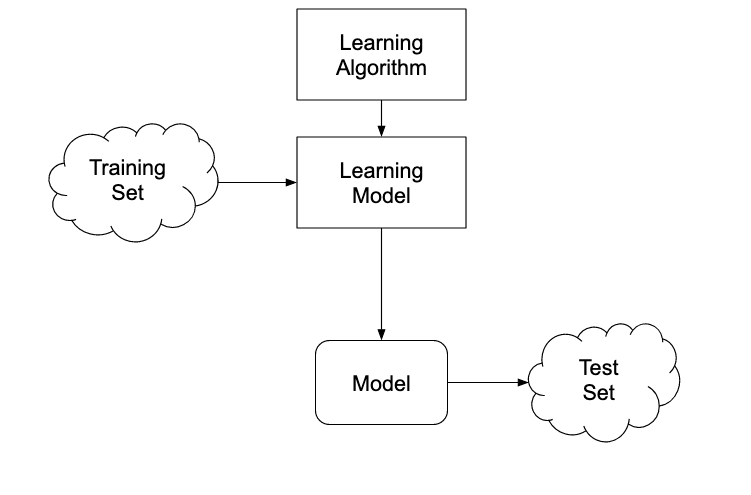
\includegraphics[scale = 0.3]{Images/classification.png}
 \caption{Generalised approach to classification problem}
 \label{fig:class}
\end{figure}
Most classification models follow a similar approach, which is detailed in Figure \ref{fig:class}. A model is learned by applying data in a training set to a learning algorithm, once the model is learned its accuracy is measured by applying it to some test data. If a row in the test data passes the classification threshold for a certain class, it is considered part of that class. The labels for each row of the test data is known, and the model is evaluated based on the accuracy of its prediction \cite{I2DM}.

\subsubsection{Evaluation}
Evaluation is generally based on the number of correct and incorrect labels that the model assigns to the test data. 
\begin{equation}\label{eq:acc}
 \text{Accuracy} = \frac{\text{Total Number of Correct Predictions}}{\text{Total Number of Predictions}}
\end{equation}
From the accuracy the error rate of the model is defined
\begin{equation}
 \text{Error Rate} = \frac{\text{Total Number of Incorrect Predictions}}{\text{Total Number of Predictions}}
\end{equation}
The confusion matrix helps give a more detailed overview of the performance of the model. It compares the actual labels with the predicted labels.
\begin{table}[H]
 \centering
 \caption{Confusion matrix}
 \begin{tabular}{ll|cc}
 &&\multicolumn{2}{c}{actual} \\
 &&\textbf{yes}&\textbf{no} \\
 \hline
 \multirow{2}{4em}{predicted}&\textbf{yes}& true positive & false positive\\
 &\textbf{no}& false negative & true negative\\
 \hline
\end{tabular}
\end{table}
Precision is the amount of positive predictions which were correct.
\begin{equation}\label{eq:precision}
 Precision = \frac{TP}{TP+FP}
\end{equation}
Recall is the amount of the true positive predictions are correct, also known as the sensitivity.
\begin{equation}\label{eq:rec}
 Recall = \frac{TP}{TP+FN}
\end{equation}
The F1 score is The harmonic mean of the precision and recall. Typically $\beta=1,0.5,2$ is used. 1 is equal weighting, 0.5 weights precision higher and 2 weights recall higher.
\begin{equation}
 F_\beta = (1+\beta^2)\left(\frac{precision \times recall}{\beta^2precsision + recall}\right)
\end{equation}
In their paper, P.Sangkatsanne et al. \cite{SANGKATSANEE20112227} proposed the use of decision trees in on-line network intrusion detection systems. They used a dataset that they created, called the RLD09, they used 13 probe attack types and 4 DoS attack types as well as normal data. They also found 12 essential features of network data for their uses by looking at the information gain of each feature and only keeping ones which are the most useful. Their project, however, collected the data using physical machines rather than virtualisation.

S.Peddabachigari et al. \cite{Peddabachigari} compared the use of support vector machines and decision trees in network IDS. They used the KDD99 dataset as their benchmark. They found that in general a decision tree performs better than a support vector machine and that a decision tree performs much better than a support vector machine when there is a lack of data. 

Y.Bouzida et al. \cite{bouzida} compared the use of neural networks to decision trees in network IDS. They also used the KDD99 dataset but also tried to classify new threats from the data. They found that decision trees both generalised well and could detect new attacks more efficiently than neural networks.

Because of these papers, the project will use a decision tree algorithm to implement anomaly based intrusion detection.

\subsection{Decision Trees}
Decision trees are a common classification method. Questions are asked of the attributes of a piece of data, from the answer to this question, another one is asked until the piece of data is classified \cite{I2DM}. They comprise three types of node:

\begin{itemize}
 \item \textbf{Root Node} - A node which has 0 incoming edges and at least 1 outgoing edge
 \item \textbf{Internal Node} - A node which has 1 incoming edge and 2 or more outgoing edges
 \item \textbf{Leaf Node} - A node which has 1 incoming edge and no outgoing edge.
\end{itemize}

The most important/significant feature should be chosen first to cause the biggest division in the data. The idea is to recursively choose the most important feature as the root of sub trees.
\begin{enumerate}
 \item If all remaining answers are positive or negative then the answer is positive or negative respectively
 \item If some are positive and some are negative then choose best examples to split them
 \item If there are no examples left then best which can be done is returning a default value. This is called plurality classification, it can be majority, random pick or a probability based on parent examples
 \item If there are no features left but still positive and negative examples, can do plurality classification on it.
\end{enumerate}
There are many ways to make a decision tree, each with varying levels of efficiency/accuracy. Most algorithms apply a greedy strategy which helps make optimum decisions \cite{10.5555/2380985}.
\subsection{Information and Entropy}
Entropy is the measure of information in a feature. It's a measure of uncertainty in a probability distribution. The best features split the examples into subsets which are ideally all positive or all negative \cite{10.5555/2380985}.

\begin{equation}
H(S) = \sum_{i=1}^c-p_i\log_2p_i
\end{equation}
where $p_i$ is the proportion of examples in $c_i$. This is maximum for a uniform distribution and minimum for a single point.


\subsubsection{Information Gain}
The measure of goodness of a feature A is found by measuring the reduction of entropy between the original examples, $S$ and the new subsets $S_i$ \cite{10.5555/2380985}.
\begin{equation}
 Gain(S,A) = H(S) - \sum_i \frac{|S_i|}{|S|}H(S_i)
\end{equation}
Information gain has a bias, it favours features with many values.
\subsubsection{Split Information} 
Split Information is the intrinsic information content within the features
\begin{equation}
 SplitInformation(S,A) = - \sum_{i=1}^c\frac{|S_i|}{|S|}\log_2\frac{|S_i|}{|S|}
\end{equation}
From this the gain ratio is found.
\begin{equation}
 GainRatio(S,A) = \frac{Gain(S,A)}{SplitInformation(S,A)}
\end{equation}
\subsubsection{Gini Impurity}
The probability of a classifier mislabelling a randomly selected example.
\begin{equation}\label{eq:gini}
 G(S) = \sum_{i=1}^cp_i\sum_{k \neq i} p_k \to 1-\sum_{i=1}^cp_i^2 \therefore G(S,A) = \sum_i \frac{|S_i|}{|S|}G(S_i)
\end{equation}
The feature with the lowest Gini impurity is the best feature to choose.

\subsection{Overfitting}
A decision tree is said to overfit the data if the tree has a large error on test data but a small error on training data \cite{10.5555/2380985}. This can be overcome by either stopping the growth earlier or by pruning the tree.

\subsection{Hunt’s Algorithm}
Hunt’s algorithm is an efficient algorithm to make decision trees, it is the basis of many popular algorithms such as C4.5, CART and ID3.\cite{I2DM}. The tree is grown recursively. If $D_t$ is the set of data which is at a node $t$ then the algorithm is given as
\begin{verbatim}
 1. If Dt contains data that belong the same class y, then t is 
 a leaf node labeled as y
 2. If Dt is an empty set, then t is a leaf node labeled as the
 default class
 3. If Dt contains records that belong to more than one class, use an 
 attribute test to split the data into smaller subsets. 
\end{verbatim}

\subsection{CART Algorithm}
The CART algorithm is based on forming rule sets from variables to either create classification trees or regression trees. \cite{cart} Rule variables are selected based on how they best split the data. The data is split based on this rule, and this is repeated recursively until the data is classified.

\subsection{C4.5 Algorithm}
The C4.5 algorithm is an algorithm developed by Ross Quinlan as an extension of the ID3 algorithm \cite{c4.5}. It works based on information gain. It chooses the feature that best splits the data. There are a few base cases. All examples belong to the same class, this creates a leaf of that class. None of the features provide any information gain or a previously unseen class is encountered, here a node higher up the tree is made using the expected value of the class.

\section{Types of Threats}
In this project, one of the main objectives is to classify unknown threats which may attack a network, to do this is it crucial to understand the threats and what differentiates them from both normal usage and other threats. The main four categories of threats are denial of service, probe, root to local (R2L) and user to root (U2R) attacks. This project will focus on classifying types of DoS attacks, however, the method may be repeated for any of these categories. 

\subsection{Denial Of Service}
The general aims of a DoS attack is to ensure that a service to become inaccessible to users. They require very little resources. They can either be persistent or non persistent. Persistent attack will permanently deny service as it can cause lasting damage, while non persistent will restore service after a while or on a restart \cite{anp}.

Flooding is one of the most common forms of DoS attack; a malicious user sends many packets to the target, limiting the ability of users to access the target \cite{tnstsa}. SYN flooding is a flooding attack that floods the user with TCP connection requests with no response.


\subsection{Probe}
A probe attack aims to find vulnerabilities in the network. It works by scanning IP addresses on the network looking for areas to exploit \cite{tnstsa}. A port scan scans each host looking for open ports to access, common ports may be the SSH port (22) or the http port (80)

\subsection{User to Root}
A user to root attack will happen once the attacker has gained access to the target machine. A user to root attack will aim to elevate the attackers’ user level privilege to root. The elevation is done using a backdoor, there are three types of backdoor: active, passive and attack based \cite{tnstsa}.

\subsection{Root to Local}
Root to local attacks attempt to gain access to the target machine, appearing as a local user of that machine. Once access is gained the user is able cause a lot of harm as they appear to be legitimate users of the network. 


